%% thesis.tex
%% Distributed with umalayathesis v1.3 (16 September 2017)
\documentclass[english]{umalayathesis}

\usepackage{lipsum}
\usepackage[utf8]{inputenc}
\usepackage[T1]{fontenc}
\usepackage{microtype}
\usepackage{graphicx}
\usepackage{xcolor}

% Useful for including code listings
\usepackage{listings}
\lstset{basicstyle=\ttfamily\SingleSpacing,
        columns=fullflexible,
        breaklines,breakatwhitespace}

% Useful for multi-page pages. Either longtable or supertabular is fine; choose any one that you're comfortable with
\usepackage{longtable}
\usepackage{supertabular}

% Sept 18, 2018 : Yousoff - Faculty require the first page of submission paper if we have published in ISI journal.
% Change subcaption to normal size
\usepackage{pdfpages}
\subcaptionsize{\normalsize}


% If your faculty requires captions to be 11pt, and only the Figure X: and Table Y: to be bold:
% \captionnamefont{\small\bfseries}
% \captiontitlefont{\small}

% If your faculty requires a ``header row'' at the top of the List of Figures/Tables:
% \addtocontents{lof}{\noindent\figurename\hfill Description\hfill Page\par}
% \addtocontents{lot}{\noindent\tablename\hfill Description\hfill Page\par}

% Sept 18, 2018 : Yousoff - Faculty require abstract in malay
% Faculty require department name
\author{Lim Lian Tze}
\title{Research Title in English}
\mtitle{Research Title in Malay}
\faculty{Faculty of Science}
\submissionyear{2017}
\degree{Master of Science}
\department{Institute Of Mathematical Sciences}

% load acronym definitions from separate file
\loadglsentries{myacronyms}
\glsaddall
%\setlength{\glsdescwidth}{.7\textwidth}

% Sept 18, 2018 : Yousoff - For your references. 2017 guidelines
%Thesis guideline	http://fs.um.edu.my/docs/librariesprovider3/PDF/mh-15-9-2017-guidelines-for-preparation-of-research-project-dissertation-and-thesis-2017-(1).pdf
%APA guideline	http://fs.um.edu.my/docs/librariesprovider3/PDF/apa-guide.pdf?sfvrsn=2
%Word template	https://www.um.edu.my/docs/librariesprovider80/students-current-students-thesis/thesis-amp-dissertation-ms-word-template-2017.docx?sfvrsn=2


\begin{document}
\frontmatter

%% Choose only ONE from the following to get the
%% correct statement on the title page
% \makecoverandtitlepage{\mastercoursework}
% \makecoverandtitlepage{\mastermixedmode}
\makecoverandtitlepage{\masterresearch}
% \makecoverandtitlepage{\doctoralcoursework}
% \makecoverandtitlepage{\doctoralresearch}
% \makecoverandtitlepage{\doctoralmixedmode}

\declarationpage
\abstractfromfile{sample-abstract}
\msabstractfromfile{sample-msabstract}
\acknowledgements{Thanks guys. I owe you many.}

% Sept 18, 2018 : Yousoff - Faculty require single spacing for all list
{\clearpage
\tableofcontents\clearpage
{
\SingleSpacing
\listoffigures\clearpage
\listoftables\clearpage
\listofacronyms\clearpage
}
\listofappendices\clearpage}

\mainmatter

\input{sample-chap-intro}
%!TEX ROOT = thesis.tex
\chapter{Dummy Chapter}

\section{Section 1} \label{chap-dummy-section-1}

\lipsum[1]. Refer to Figure \ref{fig-sample-image}. Refer to Table \ref{table-sample-table}.

\begin{figure}[ht!]\centering

\includegraphics{asset/green}
\caption{Short caption}
\label{fig-sample-image}
\end{figure}

\begin{figure}[ht!]\centering
Test 3
\caption{Long caption. Lorem ipsum dolor sit amet, consectetuer adipiscing elit. Aenean commodo ligula eget dolor. Aenean massa. Cum sociis natoque penatibus et}
\end{figure}

\begin{figure}[!ht]\centering
	\centering
	\subbottom[Subfigure 1]{%
		
\includegraphics[width=5cm]{asset/green}}
	\subbottom[Subfigure 2]{%
		
\includegraphics[width=5cm]{asset/green}}
	\caption{Multiple figure} 
	\label{fig-sample-image-2}
\end{figure} 

\begin{table}[!ht] \centering
	\caption{Short caption.}
	\begin{tabular}{|l|l|l|} \hline
		\textbf{Header 1} & \textbf{Header 2} & \textbf{Header 3} \\
		Row 1 & Row 2 & Row 3 \\ \hline
		Row 1 & Row 2 & Row 3 \\ \hline
		Row 1 & Row 2 & Row 3 \\ \hline
	\end{tabular}
	\label{table-sample-table}
\end{table}

\begin{table}[!ht] \centering
	\caption{Long caption. Lorem ipsum dolor sit amet, consectetuer adipiscing elit. Aenean commodo ligula eget dolor. Aenean massa. Cum sociis natoque penatibus et}
	\begin{tabular}{|l|l|l|} \hline
		\textbf{Header 1} & \textbf{Header 2} & \textbf{Header 3} \\
		Row 1 & Row 2 & Row 3 \\ \hline
		Row 1 & Row 2 & Row 3 \\ \hline
		Row 1 & Row 2 & Row 3 \\ \hline
	\end{tabular}
	\label{table-sample-table-2}
\end{table}

\section{Section 2}

\lipsum[1]. Refer to Section \ref{chap-dummy-section-1}. Always use shortcite \shortcite{audibert:2004}



\bibliography{myrefs}

% Make sure you have defined your own papers in the .bib file!
% Sept 18, 2018 : Remember to bold your name in the generated own.bbl
\nociteown{Lim:2009}
\bibliographyown{myrefs}

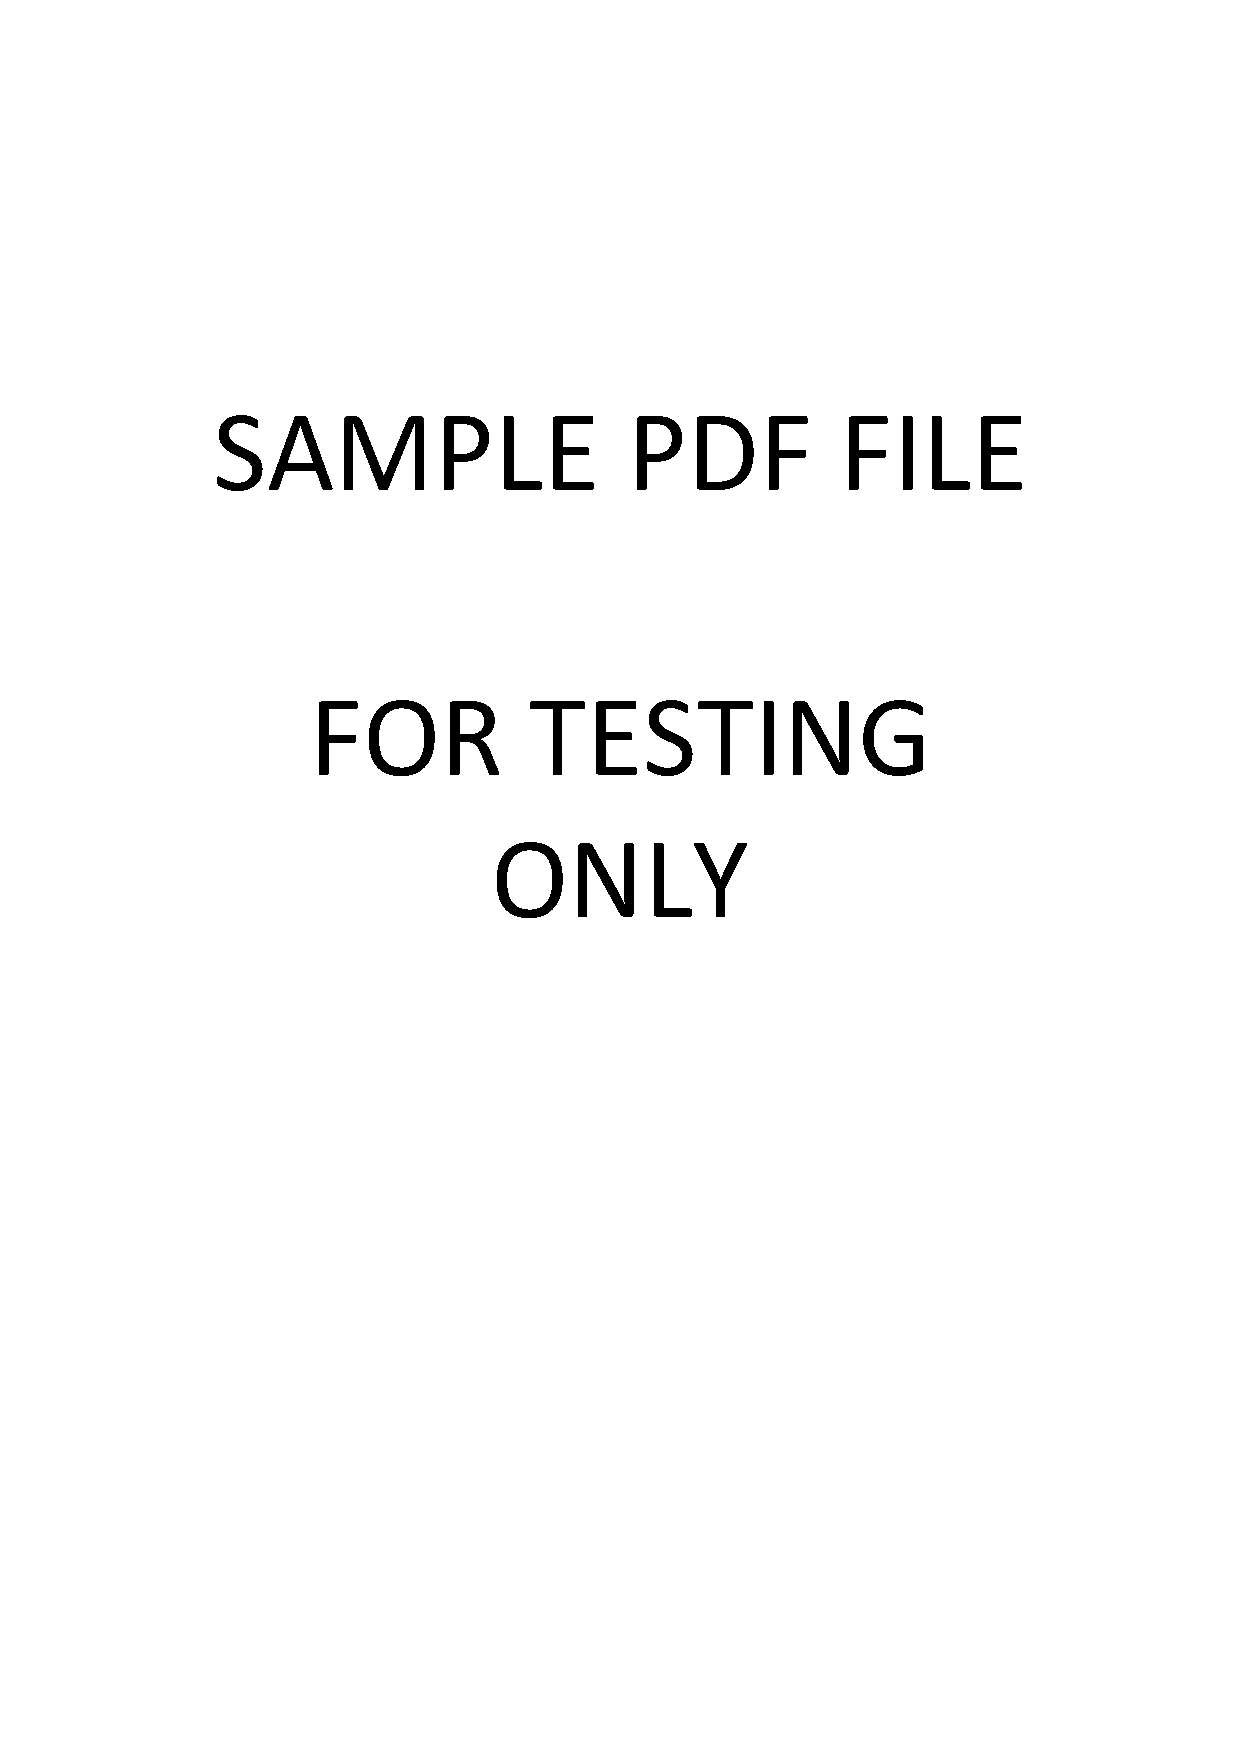
\includepdf[pages={1},pagecommand={},width=\textwidth]{asset/PDF_FILE.pdf}

\begin{appendices}
\startapps
\input{sample-appen-manual}
\input{sample-appen-try}
\finishapps
\end{appendices}

%% Comment out this line if you do not have a separate glossary.
% \printglossary

\end{document}
